
Alguns estudos sugerem que pouco mais da metade do esforço utilizado para o desenvolvimento de software
esteja voltado para atividades voltadas para assegurar a qualidade de software. Dois dos recursos utilizados como
forma de buscar o desenvolvimento de software com qualidade são a utilização de processos de desenvolvimento
de software e a utilização de padrões. Softwares que não utilizam padrões de projeto tendem a ter sua qualidade
questionável, já que os padrões garantem código bem feito, facilidade na manutenção, evolução do código sem
grandes problemas e cobertura aceitável de código.

A norma ISO/IEC 9126 foca na qualidade do produto de software, propondo Atributos de Qualidade,
distribuídos em seis características principais, com cada uma delas divididas em sub-características, conforme
podemos ver na figura abaixo:
\begin{figure}[h]
	\centering
	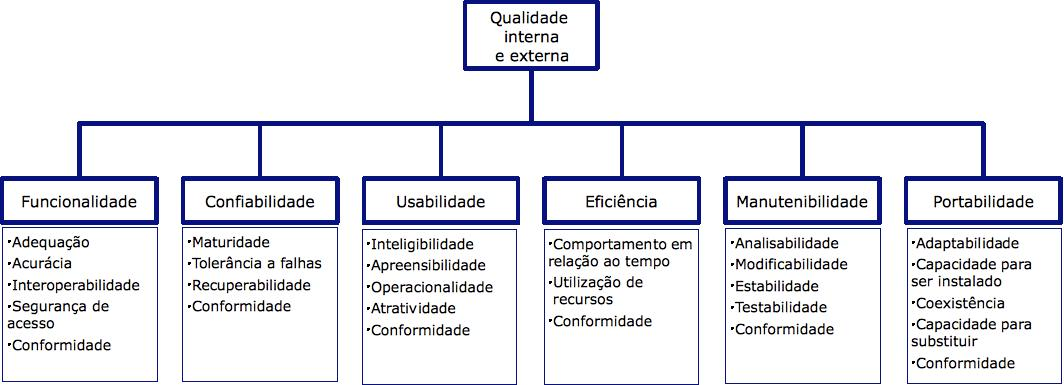
\includegraphics[width=0.8\textwidth]{conteudo/qualidade}
	\caption{Qualidade de Software\\Fonte: ISO/IEC 9126\cref{imagem}}
\end{figure}

A partir deste conceito de qualidade, procuramos obter a comparação entres sistemas que utilizam padrões
de projeto e sistemas não utilizam. O sistema de gerenciamento de clinicas de Psicologia, \textit{GestorPsi}, foi de-
senvolvido por alunos da Universidade de Brasília de forma não padronizada ou até mesmo gerenciada. Dessa
forma, as medições apresentadas farão uma comparação com medições feitas após a utilização do sistema em
uma disciplina da Universidade para manutenção e evolução do software. Durante a utilização do mesmo na
disciplina de Manutenção e Evolução de Software, padrões de projeto serão aplicados ao sistema com o objetivo
de melhorar a qualidade do software.

Os resultados esperados após esta comparação, são provas de que a aplicação de técnicas de programação,
padronização de projeto e utilização de testes de código garantem a melhoria na qualidade do software. Espera-
se obter a diferença na qualidade do software sem padronização, utilização de técnicas de programaçaõ e com
testes de código pobres e o mesmo software utilizando todos estes meios que buscam a qualidade do mesmo. A
partir deste resultado, poderemos provar que estes itens garantem uma maior qualidade do software.

